1번 예제 테스트 케이스를 봐보자

\begin{center}

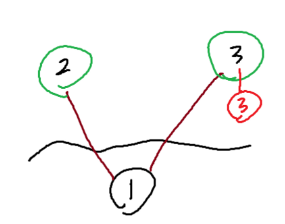
\includegraphics[bb=0 0 100 200]{1img.png}

\end{center} 
최초 트리의 형태이다. 첫 번째 쿼리시 1번을 흔들면 2, 3번 정점이 같이 흔들리고 3번 정점에 달린 열매를 떨어트리기 위해 3의 힘으로 흔들어야 한다.

\begin{center}

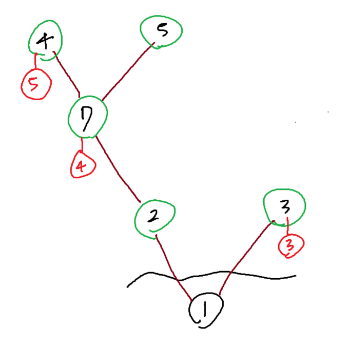
\includegraphics[bb=0 0 100 200]{2img.png}

\end{center} 
3개 접목을 진행한 모습이다. 4번을 흔들면 4번만 흔들리고, 4번에 달린 열매를 떨어트리기 위해 5의 힘으로 흔들어야 한다.
마찬가지로 7번을 흔들면 7, 4, 5번이 흔들리고 4번과 7번의 열매를 떨어트리기 위해 9의 힘으로 흔들어야 한다.

2번 예제를 봐보자
\begin{center}

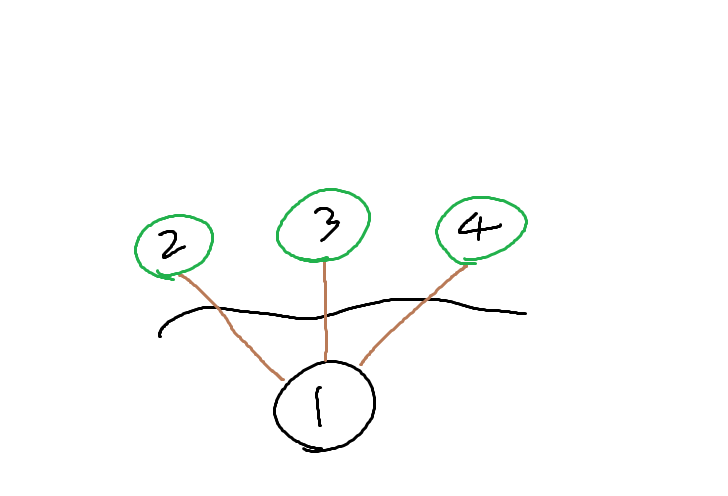
\includegraphics[scale=0.5]{3img.png}

\end{center} 
최초 트리의 형태이다. 첫 번째 쿼리시 1번을 흔들면 2, 3, 4번이 같이 흔들리지만, 열매가 달려있지 않다. 흔들어야 할 힘이 0이기에 -1을 출력한다.
\begin{center}

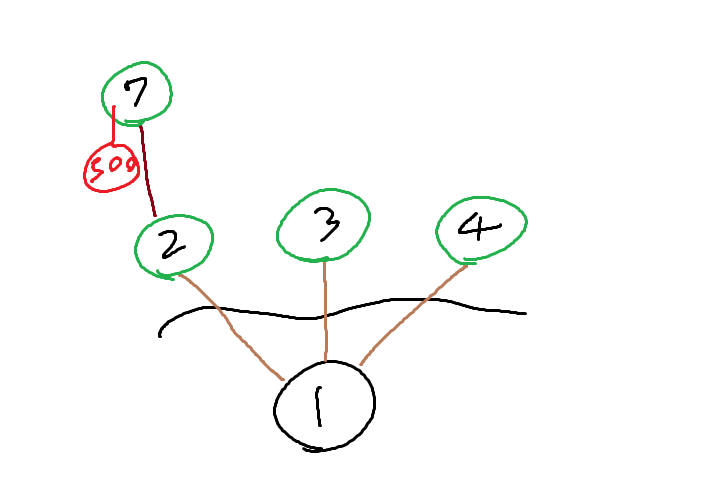
\includegraphics[scale=0.5]{4img.png}

\end{center} 
1개 접목을 진행한 모습이다. 1번을 흔들면 2, 3, 4, 7번이 같이 흔들리고, 7번의 열매를 떨어트리기 위해 500의 힘으로 흔들어야 한다.
